This page shows the details of a course.

It also provides buttons to access the corresponding chatroom and book a meeting with the professor.

\begin{figure}[H]
    \centering
    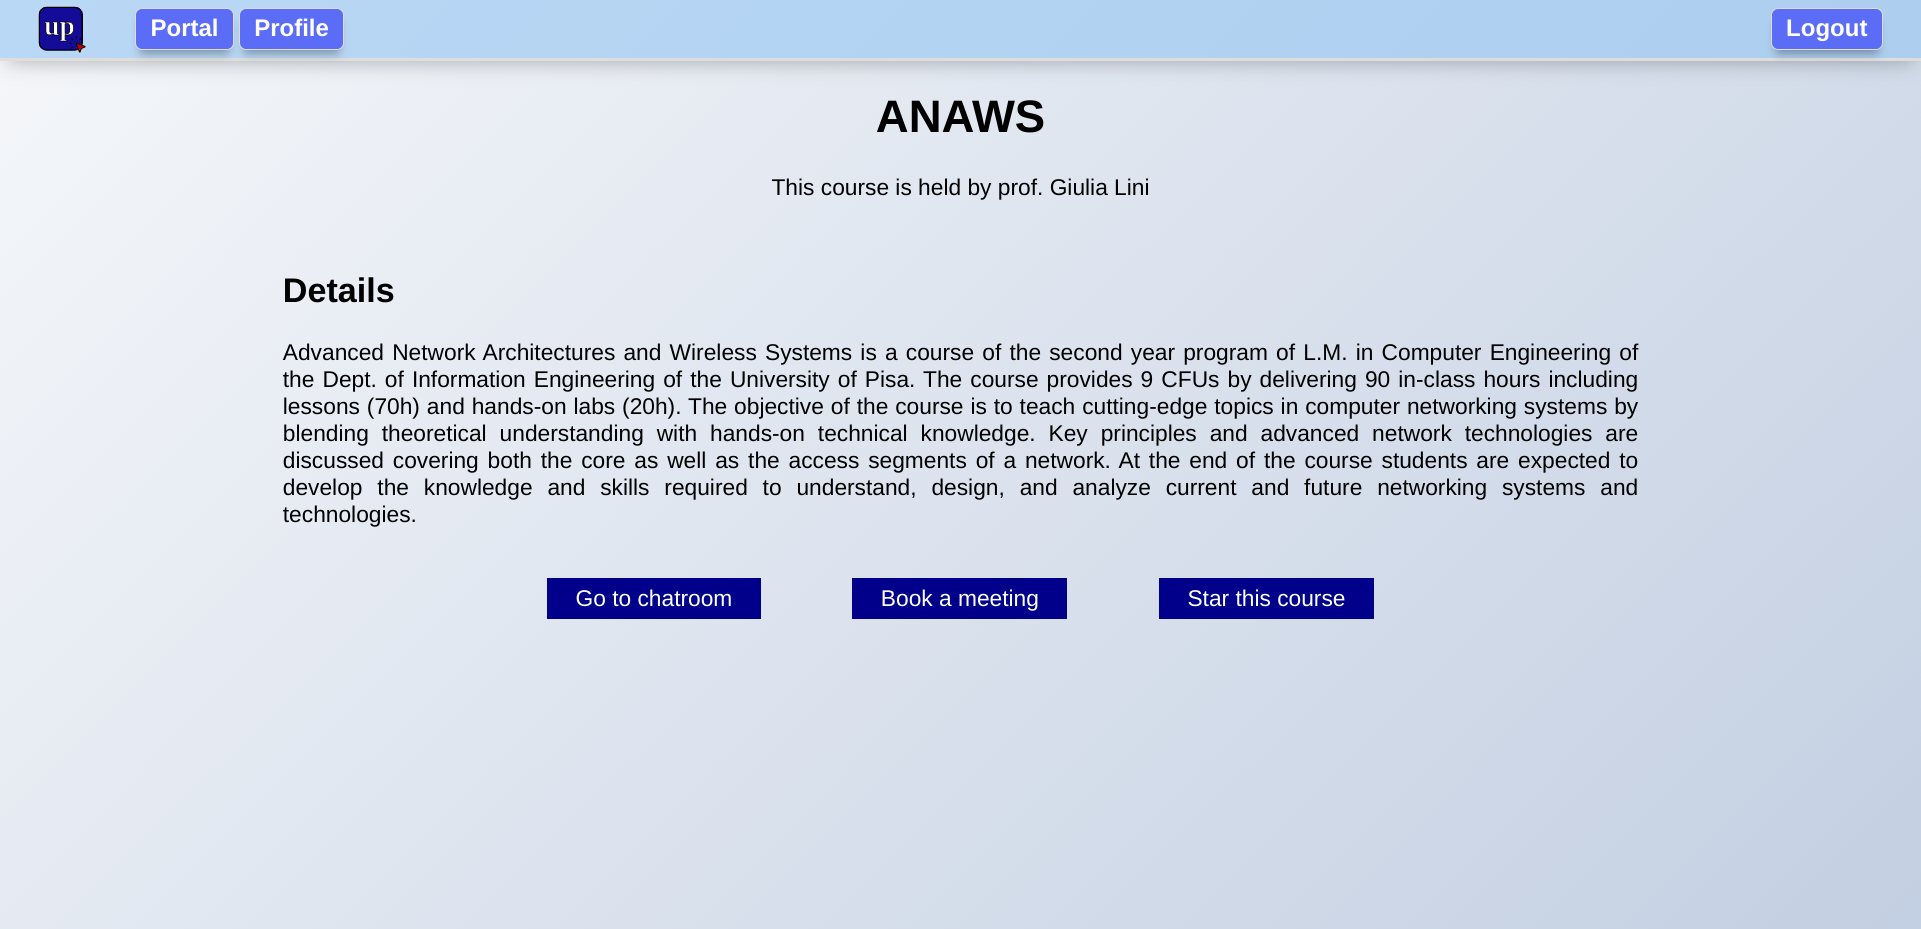
\includegraphics[width=\textwidth]{img/user_manual/student/student-course-1.png}
    \caption{Screenshot of a course page}
\end{figure}

Moreover, it is possible for a student to star the course, so that it can be shown in a separate section on their own portal page. When a student clicks on the button \textit{Start this course}, an alert pop-up spawns to notify the success of the request. The same pattern applies for the removal of a star (\textit{unstar}).

\begin{figure}[H]
    \centering
    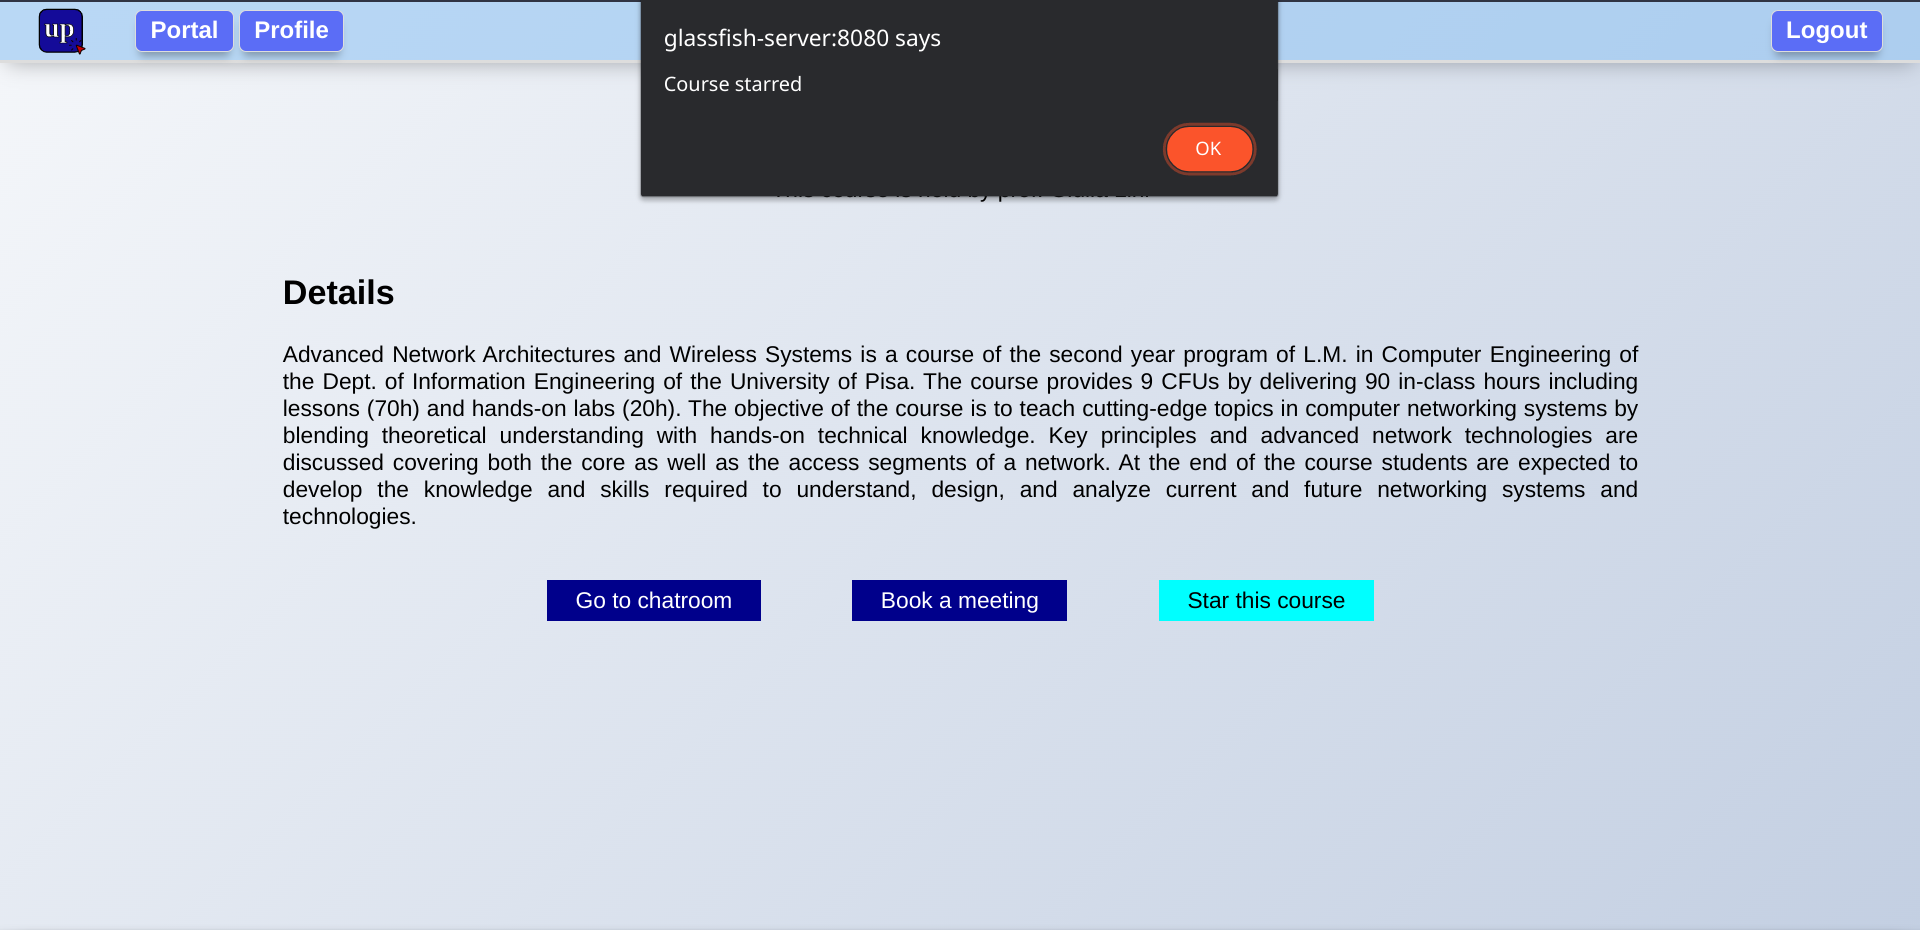
\includegraphics[width=\textwidth]{img/user_manual/student/student-course-2.png}
    \caption{Screenshot of a course page showing the alert pop-up which notify that \textit{the course has been successfully starred}}
\end{figure}
